\section{Vorwort}
Dies ist die technische Dokumentation des Projekts im Modul Programmiertechnik von Daniel Raab und Konstantin Schmidt. Es wird der Aufbau der Software beschrieben und dargestellt, sowie die einzelnen Teilmodule. Das Projekt wurde für das \emph{MSP Education Board 3.0} der HTWK Leipzig entworfen und implementiert. Der Quellcode wurde in C mithilfe des \emph{Code Composer Studio 6} geschrieben.
\section{Struktur}
\subsection{Grundstruktur}
\label{sub:grundstruktur}
Das Programm besitzt keinen sequentiellen Ablauf, da ein auf Interrupts (engl. Unterbrechungen) basierender Ansatz gewählt wurde, um alle Funktionen gut implementieren zu können.
\begin{figure}[h]
    \centering
    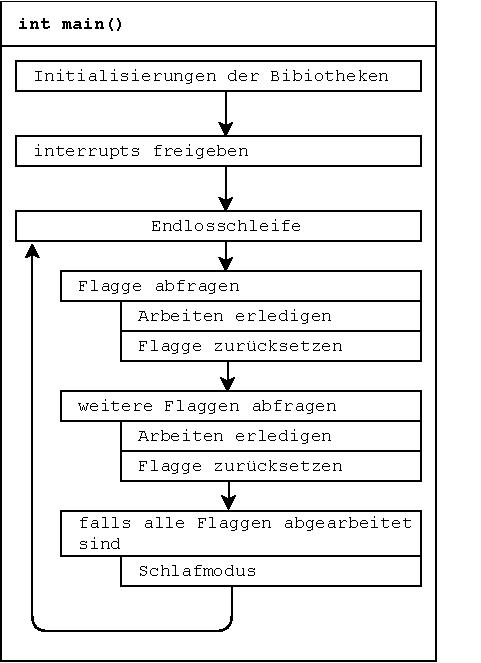
\includegraphics{main_diagram.pdf}
    \caption{Der Grundablauf schematisch dargestellt}
    \label{img:grundablauf}
\end{figure}
\newline
Der Grundablauf ist in Abbildung \ref{img:grundablauf} zusehen. Es wird zuerst der Mikrorechner und alle benötigten Systeme initialisiert und dann in den Interrupt-gesteuerten Betrieb übergegangen. Der Prozessor wird also in den Schlaf- bzw. Low-Power-Modus versetzt und reagiert ab sofort nur noch auf auftretende Interrupts. Die aufgerufene Interrupt Service Routine (ISR) soll möglichst schnell abgearbeitet werden, also wird meist lediglich das Interrupt ausgewertet und dann eine entsprechende Flagge gesetzt. Dann wird der Schlafmodus verlassen und die ISR beendet. Durch das Verlassen des Schlafmodus werden nun in der \source{main()}-Funktion die nächsten Befehle ausgeführt. Hier werden nun die Flaggen abgefragt und die entsprechenden Arbeiten erledigt. Sobald alle Flaggen abgefragt und abgearbeitet sind, wird der Prozessor wieder in den Schlafmodus versetzt. Diese Abarbeitung in der \source{main()}-Funktion hat den großen Vorteil, dass lang andauernde Arbeiten, wie z.B. Ansteuerung des Displays mit Wartezeiten, durch Interrupts unterbrochen werden können, ohne dass erst auf die lange andauernden Anweisungen gewartet werden muss. Diese Blockierung der schnell abzuarbeitenden ISRs passiert, wenn alle Aufgaben in ISRs passieren und nicht in der \source{main()}-Funktion. Zeitkritische Aufgaben z.B. Tastendrücke oder Töne könnten nicht richtig oder zeitnah ausgelesen bzw. ausgegeben werden. Eine Ausnahme dieser Regel betrifft die \source{play\_tone}-Funktion der Tonbibliothek, siehe Abschnitt \ref{sub:ton}.%TODO: ref

\subsection{Modulstruktur}
Die Programmierung des Mikrorechners erfolgte in Teilmodulen, die sich den verschiedenen Teilbereichen des Projekts widmen. Diese Teilmodule des Projekts wurden erst für sich entwickelt und sobald ein passabler Grad der Implementierung erreicht wurde in das Gesamtprojekt eingebunden und im Verbund getestet. Das Projekt wurde in folgende Module zerlegt:
\begin{itemize}
    \item Sequenz-Datenstrukturen (\textsl{sequence.h})
	\item Display-Ansteurung (\textsl{lcd.h})
	\item Eingaben, also Taster und Drehgeber (\textsl{input.h})
	\item Tonerzeugung (\textsl{tone.h})
	\item LED-Matrix (\textsl{led\_matrix.h})
\end{itemize}
Die Steuerung des Programms passiert in der \textsl{main.c} über die Funktionen, die auf die Eingaben des Benutzers reagieren. Dort werden alle Bibliotheken und Module eingebunden und zum Projekt vereinigt.

\section{Module}
Hier werden die Module genauer in ihrem Aufbau und ihrer Struktur beschrieben. Die Modulnamen für die tatsächlichen Dateien sind in Klammern angegeben und umfassen die entsprechende *.h und *.c Dateien.
